\documentclass[12pt,a4paper]{article}
\usepackage[a4paper, margin=2.5cm]{geometry}\usepackage{parskip}

%Arial
\usepackage{helvet}
\renewcommand{\familydefault}{\sfdefault}
\usepackage{parskip}

\usepackage{caption}

\usepackage[backend=biber, style=numeric-comp, sorting=none]{biblatex}
\addbibresource{refs.bib}

\usepackage{graphicx, csquotes, wrapfig, tikz, pgfplots}
\pgfplotsset{compat = newest}
\graphicspath{{./pictures/}}

\usepackage[dutch]{babel}
\usepackage{csquotes}

\usepackage[hidelinks]{hyperref}

% Source - https://tex.stackexchange.com/a/7549
% Posted by yannisl, modified by community. See post 'Timeline' for change history
% Retrieved 2026-04-03, License - CC BY-SA 4.0
\usepackage{xspace}
\newcommand{\latex}{\LaTeX\xspace}


\binoppenalty=100000
\relpenalty=100000



\title{Het magnetisch veld van de Aarde}
\author{Tjalling, Leonetti \and  Aron, Martens \and Ijmert, Ulens  \and Olaf, Van Tichelen }
\date{
  Algemene Natuurkunde II (B-KUL-G0N13B) \\
  22 mei 2026}
\begin{document}
\maketitle
\tikz[remember picture, overlay]{
  \node[anchor=north east] at (current page.north east) {
    
\includegraphics[scale=0.5]{kul_logo}
  };
}

\begin{figure}[b!]
  \centering
  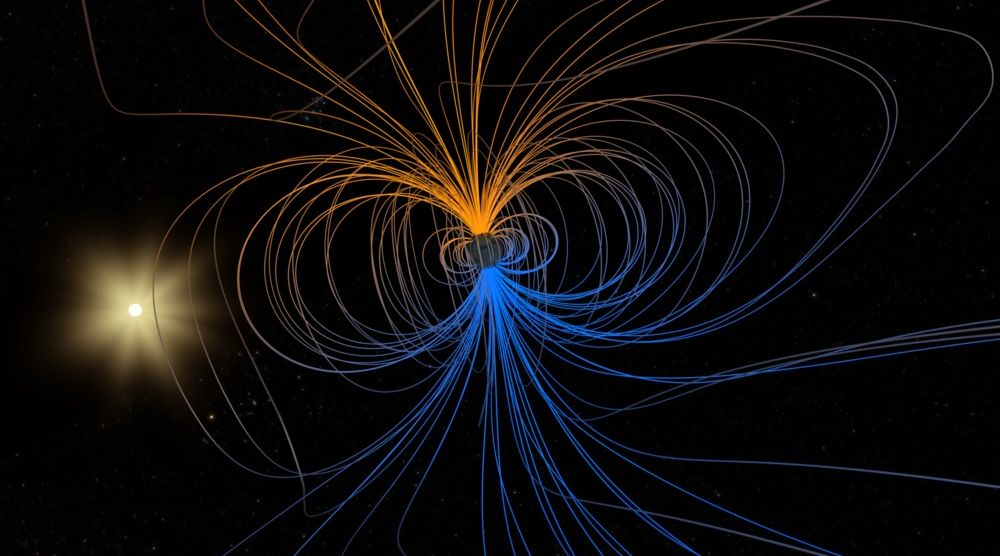
\includegraphics[width=\textwidth]{magnetic_field_cover_print.jpg} %TODO: IMAGE
  \caption*{Voorbeeld voorblad: TODO \cite{voorblad}}
\end{figure}
\newpage
\tableofcontents

\newpage
\section{Inleiding}
\section{Huidige structuur van het magneetveld \texorpdfstring{\&}{&} mechanismen die dit instand houden}
\label{sec:sec_2}

Ondanks het feit dat de aarde een magneetveld heeft, met allerlei alledaagse toepassingen, wordt het vaak slecht begrepen. Historisch gezien is de belangrijkste toepassing van het magneetveld navigatie.
Zo weet men bijvoorbeeld dat in de 1ste eeuw n.C. in China een soort kompas werd uitgevonden, bestaande uit een zeilstenen lepel, waarvan men al wist dat dit gesteente magnetisch was.
Deze lepel roteerde op een gladde plaat en richtte zich naar het magnetisch noorden \cite{aron_book_ch1}. Ook beschermt het magnetisch veld ons tegen de zonnewind.
Dit is een stroom geladen deeltjes afkomstig van de zon, die schadelijk zou zijn voor het leven op aarde \cite{aron_book_ch2}. Het magnetisch veld heeft een meetbare structuur en een fysieke oorsprong.
Deze zullen allebei aan bod komen in dit hoofdstuk. We zullen nu starten met de eenvoudigste beschrijving van deze structuur.

Een eerste benadering voor het magneetveld van de aarde is die van een eenvoudige staafmagneet, ofwel een dipool. Hierbij komen de veldlijnen tevoorschijn in de ene pool, bewegen zich gekromd voort door de ruimte en verdwijnen weer in de andere pool, zoals te zien is in Figuur \ref{fig:aron1} \cite{aron_book_ch2}. %TODO:HEREE 
Dit geeft ons een notie voor een magnetische noord- en zuidpool, maar deze zijn anders dan de geografische polen van de aarde, het aardmagnetisch veld heeft een dipoolrichting die 11° gekanteld is ten opzichte van de rotatieas \cite{aron_book_ch2, aron_demorest_paper}.
Dit model geeft ons ook een beeld van de sterkte van het veld. Zo zien we in Figuur \ref{fig:aron1} dat de veldlijnen aan de polen dichter bij elkaar liggen en het veld dus sterker is dan aan de evenaar.
Deze manier om het magneetveld van de Aarde te beschrijven volstaat om de algemene structuur die we observeren te beschrijven, maar hoewel het dipoolmodel een goed statisch beeld geeft, verklaart het niet waar het magneetveld vandaan komt en of het stabiel is.

\begin{figure}[hbt!]
    \centering
    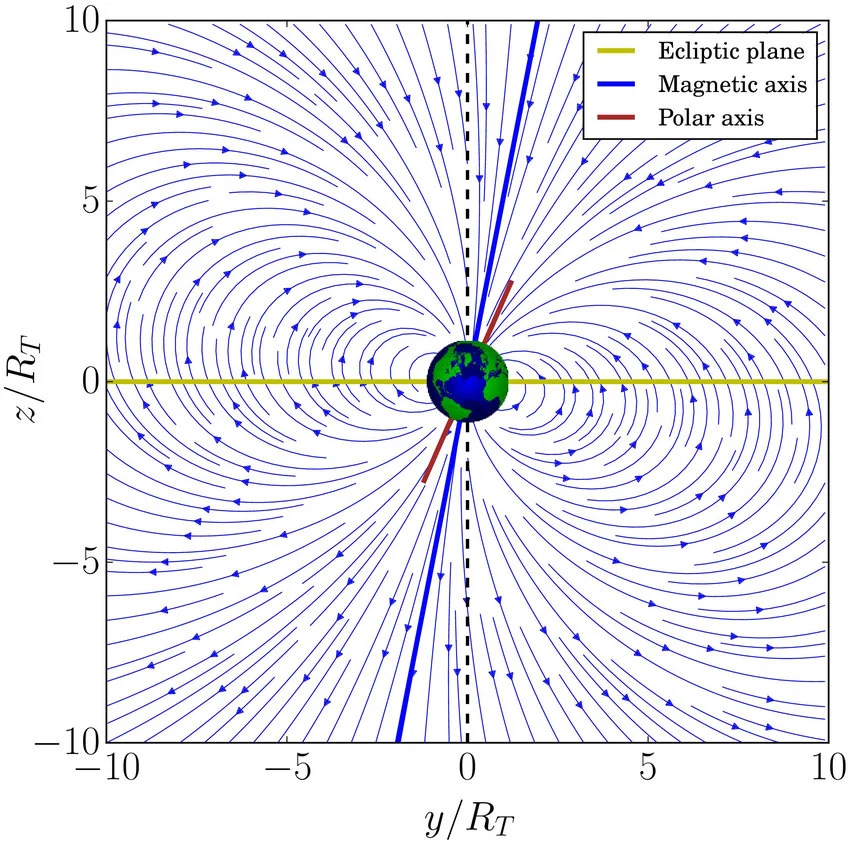
\includegraphics[width=0.5\textwidth]{aron1.jpg}
    \caption{visuele voorstelling van veldlijnen van het statische dipoolveld \cite{aron_image1}}
    \label{fig:aron1}
\end{figure}

Het voornaamste bewijs waarom het dipoolmodel tekort schiet is terug te vinden in gesteenten. Ijzer en andere gesteenten leggen namelijk hun magnetische oriëntatie vast wanneer ze voorbij hun Curiepunt afkoelen. Dit vormt de basis voor het paleomagnetisme \cite{aron_demorest_paper}.
Zo weet men uit waarnemingen dat het magneetveld niet altijd hetzelfde geweest is. Het veld ondergaat herhaaldelijke polariteitswisselingen, wat fundamenteel incompatibel is met een statisch dipoolmodel \cite{aron_demorest_paper}. Paleomagnetisme en andere modernere technieken om veranderingen in het veld waar te nemen worden verder besproken in \hyperref[sec:sec_4]{Hoofdstuk 4}.

\begin{figure}[h!]
    \centering
    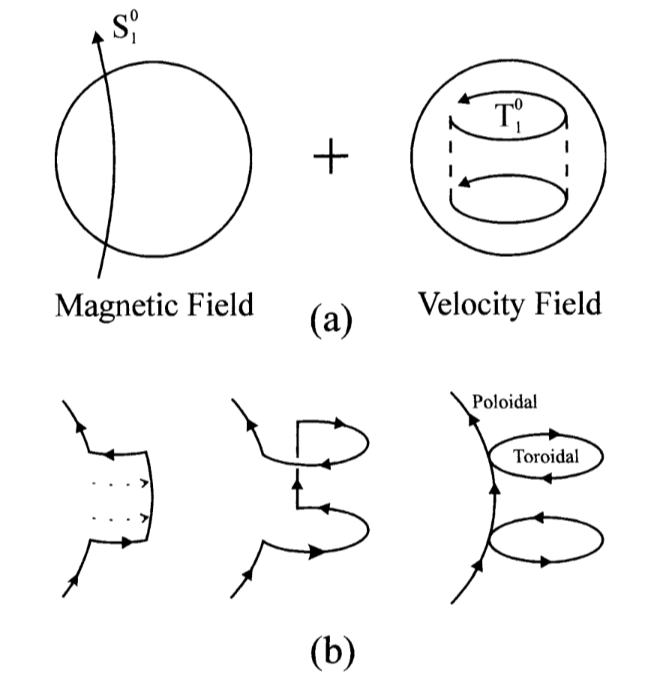
\includegraphics[width=0.5\textwidth]{aron2.png}
    \caption{Visuele voorstelling van hoe het $\omega$-effect het poloidale veld toroidaal maakt in de aardkern. (a) Een initieel magneetveld dat door de kern gaat (links) en een cylindrisch snelheidsveld (rechts) worden weergegeven. (b) De interactie tussen beide velden in (a) wordt op drie verschillende momenten weergegeven, van links naar rechts \cite{aron_book_ch8}}.
    \label{fig:aron2}
  \end{figure}
De antwoorden op de vragen over het aardmagnetisch veld zijn te vinden binnenin de aarde. Het vaste binnenste deel van de kern en het vloeibare buitenste deel bestaan beide voornamelijk uit ijzer. Aangezien ijzer geleidend is, wordt een elektrisch veld opgewekt wanneer deze vloeistof door het magneetveld beweegt, wat op zijn beurt een nieuw magneetveld opwekt \cite{aron_demorest_paper}.
Dit biedt de basis voor de dynamotheorie, ook wel de magnetohydrodynamica (MHD) genoemd. Er zijn twee zaken die dit proces stabiel houden.
Enerzijds is er het $\omega$-effect. Dit effect vindt plaats doordat de vloeistof sneller circuleert op sommige diepten dan andere, waardoor het de veldlijnen buigt en keert van een poloidale naar een toroidale configuratie, zoals te zien is in Figuur \ref{fig:aron2} \cite{aron_demorest_paper, aron_book_ch8}. Anderzijds speelt het $\alpha$-effect een rol.
Dit effect beschrijft hoe opstijgende kolommen vloeistof beïnvloed worden door de Corioliskracht, waardoor het toroidale veld weer omgezet wordt naar het originele poloidale veld \cite{aron_demorest_paper, aron_book_ch8}. Deze effecten worden samen het $\alpha\omega$-effect genoemd.
De nodige energie voor deze effecten wordt geleverd door het stollen van de binnenkern, waardoor warmte en lichtere elementen vrijkomen, die de vloeistofstromen aanwakkeren \cite{aron_demorest_paper}. Verder is deze dynamo ook wel echt noodzakelijk voor ons magneetveld.
De berekeningen in \cite{aron_book_ch8} laten immers zien dat het magneetveld zonder dynamo zou uitdoven na 10 000 tot 30 000 jaar. Aangezien de aarde veel ouder is dan dit, biedt dit nog een bewijs dat een dynamotheorie niet onredelijk is.
Het $\alpha\omega$-effect is stabiel genoeg om op korte tijdschaal een dipool voor te stellen, maar ook chaotisch genoeg om polariteitsomkeringen te verklaren.

Omdat de geodynamo chaotisch is, is het niet praktisch om de volgende polariteitsomkeringen deterministisch te voorspellen. Hiervoor worden twee moderne aanpakken gebruikt.
De eerste methode is het stochastisch modelleren van het magneetveld door gebruik te maken van paleomagnetische observaties en verzamelde data. Hieruit krijgt men allerhande resultaten, zoals dat de kans op een omkering in de komende 20 000 jaar kleiner dan 2\% is en dat de huidige afname in dipoolmoment vreemd is, maar wel nog binnen de natuurlijke variatie valt \cite{aron_next_reversal}.
De andere methode is de volledige MHD vergelijkingen numeriek te simuleren. Zo zijn Glatzmaier \& Roberts er in 1995 al in geslaagd om een veld zoals dat van de Aarde te simuleren, dat ook spontane omkeringen onderging \cite{aron_roberts}. Deze methoden vullen elkaar aan en hebben elk hun voor- en nadelen en naar beide wordt nog steeds onderzoek gevoerd.


\section{Hoe het aardmagnetisch veld kan worden gemeten}
Een bekend meetinstrument om het aardmagnetisch veld te meten is de fluxgate magnetometer.
Het eerste onderdeel daarvan is een zacht magnetisch materiaal dat de vorm van een ring heeft dat fysici de kern noemen.
Een zacht magnetisch materiaal is een materiaal dat zich in de buurt van een magneetveld magnetiseert maar wanneer het magneetveld verdwijnt weer demagnetiseert zoals weekijzer.
Een aandrijfspoel is rond de hele ring gewikkeld waarbij denkbeeldig de linkerkant en de rechterkant van de ring worden onderscheden.
Rond de ring met de aandrijfspoel zit een grotere detectiespoel gewikkeld zoals in Figuur \ref{fig:tjalling1}.
\begin{figure}[hbt!]
    \centering
    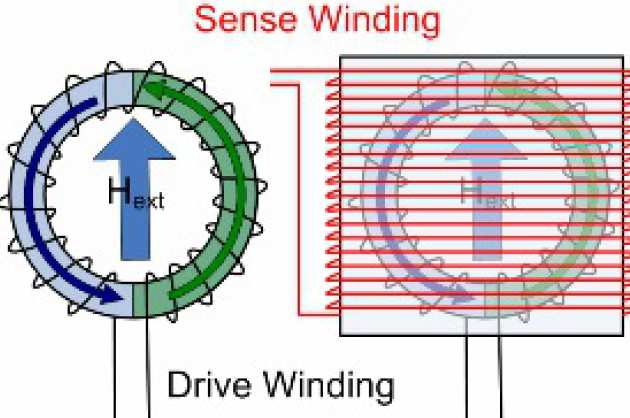
\includegraphics[width=0.5\textwidth]{tjalling_fig1.jpg}
    \caption{}
    \label{fig:tjalling1}
\end{figure}
Op de aandrijfspoel zit een wisselstroom. Beide kanten van de spoel zullen een magneetveld produceren waardoor de kern zich magnetiseert.
Iedere helft van de kern zal daardoor voor een fluxverandering in de detectiespoel zorgen.
Op een gegeven moment zal de kern zich niet nog meer magnetiseren.
Zelfs niet als het magnetisch veld veroorzaakt door de stroom van de aandrijfspoel groter wordt.
Dat noemen fysici verzadiging. Indien er geen extern magnetisch veld is, creëren de twee kanten van de kern voor de verzadiging een tegengestelde fluxverandering in de detectiespoel.
De verzadiging is voor de twee kanten van de kern dan ook op exact hetzelfde moment. De totale fluxverandering in de detectiespoel zal daardoor altijd gelijk aan nul zijn.
Volgens de inductiewet van Faraday zal de detectiespoel dan geen spanning krijgen.
Indien een extern magnetisch veld een component heeft die uniform door de detectiespoel gaat, hebben beide helften van de kern zich al gemagnetiseerd.
Het magnetisch veld is voor de ene helft van de kern in dezelfde zin en voor de andere helft van de kern in de tegengestelde zin van het magnetisch veld dat veroorzaakt is door de aandrijfspoel en door hen gaat.
Wanneer de aandrijfspoel de twee helften magnetiseert, is het alsof exact hetzelfde proces optreedt maar waarbij de twee helften vanaf een ander vertrekpunt starten.
Daardoor treedt de verzadiging van de twee helften niet op exact hetzelfde moment waardoor de totale fluxverandering in de detectiespoel dan niet gelijk aan nul zal zijn.
Volgens de inductiewet van Faraday zal de detectiespoel een spanning krijgen. Als een van de twee helften het eerst verzadigt zal de spanning van de detectiespoel hard stijgen.
Na een tijd raakt de tweede helft echter ook verzadigd en zal de spanning van de detectiespoel weer hard naar nul dalen.
Omdat de stroom van de aandrijfspoel een wisselstroom is, zal daana exact hetzelfde proces maar dan met een negatieve spanning optreden.
Het gevolg is dat de spanning van de detectiespoel een wisselspanning is. Anders gezegd is de spanning van de detectiespoel in functie van de tijd een sinusfunctie.
Fysici meten de amplitude van die functie. Ze berekenen daarmee het component van het aardmagnetisch veld dat door de detectiespoel gaat.
De fluxgate magnetometer blijkt een zeer gevoelig instrument te zijn dat waarme fysici waarden van tot de nanotesla exact bekomen.
Het probleem is echter dat maar een component van het aardmagnetisch veld werd gemeten. Een oplossing is om op het punt waar het gewenst is het aardmagnetisch veld te meten een orthonormale assenstelsel in te voeren.
Het component van het aardmagnetisch veld volgens de x-as, y-as en z-as is dan meetbaar door de fluxgate magnetometer volgens de x-as, y-as en z-as te leggen. 
Zo zijn de sterkte en richting van het aardmagnetisch veld makkelijk te berekenen
\cite{tjalling_imperial, tjalling_physicsopenlab, tjalling_dexinmag}.

\section{Veranderingen}
\label{sec:sec_4}
Het aardmagnetisch veld is allesbehalve statisch; het verandert voortdurend van sterkte, richting en zelfs van polariteit. Door de geschiedenis van de Aarde heen hebben deze veranderingen plaatsgevonden op verschillende tijdschalen, van eeuwen tot miljoenen jaren.
Wetenschappers hebben dit fascinerende verleden kunnen bestuderen door gebruik te maken van slimme methoden die variëren van het bestuderen van oude stenen tot het analyseren van scheepsjournalen.

De meest drastische veranderingen die het magnetisch veld ondergaat, zijn de polariteitsomkeringen. Hierbij schuiven de magnetische polen over de aardbol en wisselen uiteindelijk van plaats.
Dit is geen plotselinge gebeurtenis, maar een chaotisch proces dat enkele duizenden jaren kan duren. Gedurende deze periode verzwakt het veld en wordt het instabiel, wat tijdelijk de bescherming tegen kosmische straling vermindert.
Gemiddeld zit er ongeveer 300.000 jaar tussen deze omkeringen. De laatste volledige omkering vond ongeveer 780.000 jaar geleden plaats, wat betekent dat we momenteel "over tijd" zijn voor de volgende.

De laatste 2000 jaar is het veld met 35\% afgenomen in sterkte en er zijn aanwijzingen dat het veld zich momenteel mogelijk voorbereidt op een omkering, al kan de huidige verzwakking ook onderdeel zijn van een tijdelijke fluctuatie.

Recent onderzoek uit 2026 heeft ons beeld van dit proces verrijkt. Door sedimentkernen uit de Noord-Atlantische oceaan te analyseren, ontdekten wetenschappers dat een omkering van ongeveer 40 miljoen jaar geleden maar liefst 70.000 jaar duurde.
Dit is zeven keer langer dan de eerder geschatte 10.000 jaar en bewijst dat de duur van omkeringen sterk kan variëren.

Naast deze korte "flips" zijn er ook superchrons: perioden van uitzonderlijke stabiliteit waarin het veld gedurende tientallen miljoenen jaren niet omkeert.
In de laatste 540 miljoen jaar zijn er drie van zulke superchrons bekend. Onderzoek heeft zelfs aanwijzingen gevonden voor nog eens tien superchrons in de 1,3 miljard jaar daarvoor.
Dit is verrassend omdat wetenschappers verwachtten dat de afkoeling van de Aarde en de groei van de vaste binnenkern een groot effect zouden hebben op het gedrag van het veld.
De ontdekking suggereert dat het mechanisme dat het veld opwekt, de geodynamo, veel robuuster is dan gedacht.

Omdat er niemand was om het magnetisch veld van miljoenen jaren geleden te meten, moeten wetenschappers creatief zijn.

\textbf{Paleomagnetisme}: Dit is de belangrijkste methode om ver terug in de tijd te kijken. Bepaalde gesteenten, zoals vulkanisch gesteente (basalt), bevatten ijzerhoudende mineralen (zoals magnetiet).
Wanneer lava afkoelt, worden deze mineraaltjes gemagnetiseerd in de richting van het dan heersende aardmagnetisch veld. Deze richting wordt vervolgens "bevroren" in het gesteente.
Op dezelfde manier kunnen sedimenten op de bodem van oceanen kleine magneetkorreltjes bevatten die zich tijdens afzetting als minuscule kompasnaaldjes richten naar het veld.

Een nieuwe techniek, \textbf{Micromagnetische Tomografie} (MMT) gaat nog een stap verder.
In plaats van het gemiddelde signaal van miljoenen korreltjes te meten, kan MMT het magnetische moment van individuele mineraalkorrels analyseren.
Hierdoor kunnen wetenschappers de betrouwbare signaaldragers eruit pikken en nog preciezere reconstructies maken van het oude veld.

\textbf{Archeomagnetisme}: Voor de periode van de laatste duizenden jaren biedt archeologie een uitkomst.
Voorwerpen van gebakken klei, zoals aardewerk, bakstenen of de wanden van ovens, zijn uitstekende registraties.
Tijdens het bakken verliezen de kleimineralen hun oude magnetisatie en krijgen ze bij afkoeling een nieuwe magnetisatie, exact parallel aan het veld van dat moment.
Door deze voorwerpen te bestuderen, kunnen wetenschappers het gedrag van het veld van de afgelopen millennia reconstrueren.

Historische bronnen: Het archief in scheepsjournalen: Voor de laatste 400 jaar is er nog een bijzondere bron: de logboeken van zeevaarders.
Vanaf de 16e eeuw voeren schippers op hun kompas. De afwijking tussen de door het kompas aangewezen richting en de ware geografische noordpool (de declinatie) werd nauwkeurig genoteerd.
Geofysicus Dr. Andrew Jackson reisde door Europa om duizenden van deze scheepsjournalen uit de periode 1590-1900 te lezen.
Door deze enorme hoeveelheid data te combineren met andere metingen, kon hij de veranderingen in het veld van de afgelopen eeuwen in kaart brengen. 


%
\section{Magnetische velden van planeten en de Zon}

Het magnetisch veld is niet uniek aan onze aarde. Het komt ook voor bij andere planeten, en bij onze zon. Maar ze is wel verschillend in sterkte.
Sommige planeten hebben er geen, andere hebben er die tot wel 50 keer sterker kunnen zijn dan van onze aarde. 

%TODO:rest of chapter

\section{Hoe organismen het magnetisch veld van de aarde kunnen waarnemen: magnetoreceptie}
Het vermogen om de richting en/of de grootte van magnetische velden waar te nemen duikt op in diverse organismen, van bacteriën en reptielen tot zoogdieren en vogels 
\cite{ijmert_annual_reviews, ijmert_open_life_sciences}.
Hoewel magnetoreceptie is vastgesteld bij veel verschillende organismen, is het onderliggende mechanisme voor vele ervan nog niet opgehelderd.
De zoektocht naar mechanismen en sites van magnetoreceptie in biologische wezens wordt bemoeilijkt doordat het gehele organisme als potentiële locatie in aanmerking komt.
Biologisch materiaal is namelijk grotendeels doorlatend voor magnetische velden, in tegenstelling tot zichtbaar licht bijvoorbeeld.
Hierdoor kunnen de magnetoreceptieve structuren zich eender waar in het organisme bevinden, in tegenstelling tot organen die instaan voor het waarnemen van zichtbaar licht, die kort bij het oppervlak van het organisme moeten liggen.

Een bijkomende verklaring voor de bemoeilijkte vooruitgang in de zoektocht naar magnetoreceptieve mechanismen in organismen is het gebrek aan een analoog zintuig bij de mens.
Mechanismen voor de waarneming van UV-licht door bepaalde organismen bijvoorbeeld is echter een extensie van de capaciteit van de mens om zichtbaar licht waar te nemen.
Hierdoor kan er gebruikgemaakt worden van menselijke intuïties en de grote kennis van het menselijk oog om verklaringen te achterhalen voor deze mechanismen.
Hoewel er studies bestaan die suggereren dat mensen mogelijk gevoelig zijn voor veranderende magnetische velden, is dit niet vergelijkbaar met het zicht, aangezien dat laatste een evident, bewust en uitgebreid bestudeerd zintuig is waarop menselijke intuïtie veel gemakkelijker kan steunen
\cite{ijmert_annual_reviews, ijmert_physics_today, ijmert_eneuro}.

Een voorbeeld van een organisme waarbij het mechanisme van magnetoreceptie wél is opgehelderd, zijn magnetotactische bacteriën. Al in 1963 werd waargenomen dat deze groep bacteriën zwommen in de richting van de noordpool van de aarde.
Dit gedrag wordt mogelijk gemaakt door gespecialiseerde organellen, zogenaamde magnetosomen.
Deze organellen bestaan uit een membraan omsloten ijzerbevattend kristal, met een bepaalde grootte die ervoor zorgt dat ze bestaan uit één enkel magnetisch domein en zich gedragen als een permanente magneet op kamertemperatuur.
Dit kristal zal zich oriënteren in het magnetisch veld van de aarde zodat de magnetische noordpool van het kristal naar de zuidpool van de aarde wijst. In het merendeel van de magnetotactische bacteriën zullen deze organellen samenhangen in kettingen, zoals te zien in 
Figuur \ref{fig:ijmert1}. Deze ketting zal zich oriënteren naar het magnetisch veld en zich gedragen als een kompasnaald 
\cite{ijmert_nature}.

\begin{figure}[hbt!]
    \centering
    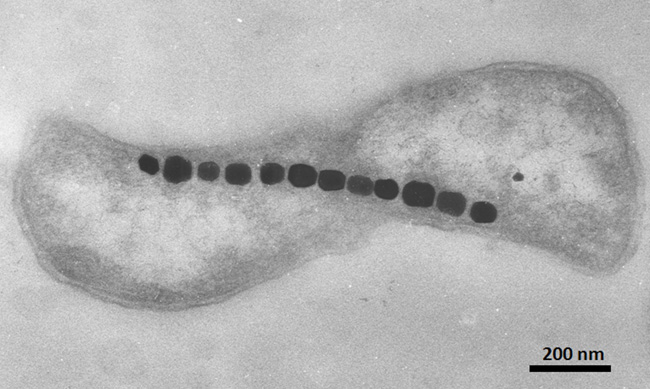
\includegraphics[width=0.5\textwidth]{ijmert_fig1.jpg}
    \caption{Magnetosoom ketting in bacterium \cite{ijmert_nature}}
    \label{fig:ijmert1}
\end{figure}
De werking van magnetoreceptie bij dieren is veel minder duidelijk dan het mechanisme voor magnetoreceptie bij de magnetotactische bacteriën. Er worden meerdere mechanismen voorgesteld, waaronder 
\cite{ijmert_physics_today}:
\begin{itemize}
  \item een gelijkaardig proces als de magnetotactische bacteriën, leunend op magnetische ijzer bevattende kristallen.
  \item magnetoreceptie leunend op elektromagnetische inductie, waar een geleidend materiaal een potentiaalverschil creëert wanneer het door een magnetisch veld beweegt.
  \item het kwantummechanische radicale-paar mechanisme, waar het magneetveld invloed heeft op de reactiesnelheid van een chemische reactie. 
\end{itemize}

Veel dieren, zoals haaien en andere vissen, hebben het vermogen om elektrische velden te detecteren.
Bij haaien leunt het mechanisme op honderden kanalen die beginnen in de poriën op de huid van de haai, en ergens in het lichaam van de haai eindigen.
De wanden van deze kanalen zijn uiterst resistief, en de kanalen zijn gevuld met een geleidende gelei achtige substantie. Wanneer de haai zwemt in een magnetisch veld, zal er een potentiaalverschil ontstaan over deze geleidende substantie.
Dit door de magnetische inductie van een geleider wanneer het beweegt door een elektrisch veld. De zintuiglijke structuren genaamd de Ampullen van Lorenzini op het einde van de kanalen in de haai, kunnen dit potentiaalverschil waarnemen.
Op deze manier is het theoretisch mogelijk om een magnetisch veld waar te nemen 
\cite{ijmert_physics_today}. 

Het mechanisme, gebaseerd op het kwantummechanische radicale-paar mechanisme, zou plaatsvinden in fotoreceptieve eiwitten, namelijk cryptochromen.
De radicale paren zullen verschillende chemische reacties ondergaan, afhankelijk van of ze zich in een singlet of triplet toestand bevinden.
De snelheid waarbij een radicaal naar een triplet toestand overgaat hangt af van het magnetisch veld, dus de aanwezigheid van het chemisch product afkomstig van de chemische reactie geassocieerd met de triplet toestand kan informatie opleveren over het magnetisch veld.
Dit mechanisme, samen met het mechanisme leunend op magnetische ijzer bevattende kristallen, zijn mogelijke verklaring voor magnetoreceptie in vogels.
Ze gebruiken magnetoreceptie om zich te oriënteren tijdens hun seizoensgebonden migratie 
\cite{ijmert_physics_today, ijmert_royal_society}.
\section{Samenvatting}

\section{Bibliografie}

\printbibliography[heading=none]
\section{AI-gebruik}

\end{document}

